\documentclass{altsu-report}
\linespread{1,15}
\title{Дребезг кнопок в устройствах персонального типа}
\author{А.\,В.~Лаптев}
\groupnumber{595}
\GradebookNumber{1337}
\supervisor{И.\,А.~Шмаков}
\supervisordegree{ст. преп.}
\ministry{Министерство науки и высшего образования}
\country{Российской Федерации}
\fulluniversityname{ФГБОУ ВО Алтайский государственный университет}
\institute{Институт цифровых технологий, электроники и физики}
\department{Кафедра вычислительной техники и электроники}
\departmentchief{В.\,В.~Пашнев}
\departmentchiefdegree{к.ф.-м.н., доцент}
\shortdepartment{ВТиЭ}
\abstractRU{Данная работа посвящена исследованию проблемы дребезга и методов ее решения.

В результате выполнения научно-исследовательской работы былпроведен анализ различных методов погашения дребезга и выбран и реализован один из них в качетсве решения для конкретного устройства -- генератора персонажа DnD.}
\abstractEN{Большой текст на английском!}
\keysRU{Дребезг, прерывание, кнопка}
\keysEN{computer simulation, distributed version control}

\date{\the\year}

% Подключение файлов с библиотекой.
\addbibresource{graduate-students.bib}

\begin{document}

\maketitle

\setcounter{page}{2}
\makeabstract
\tableofcontents

\chapter*{Введение}

Различные кнопки и переключатели встречаются в цифровой аппаратуре повсеместно, поэтому проблема дребезга контактов в них зачастую является существенной. Дребезг контактов может стать причиной неправильной работы устройства в следствие неверного распознавания переключения или нажатия/отжатия кнопки, а это в ряде случаев может стать критичным даже для человека.

Например, при использовании в медицинской или промышленной аппаратуре неправильное распознавание нажатий может стать причиной несчастного случая или ухудшения состояния здоровья человека.

\chapter{Что такое дребезг контактов и причины возникновения дребезга}

Дребезг контактов --- явление, происходящее в электромеханических коммутационных устройствах и аппаратах, длящееся некоторое время после замыкания электрических контактов~\cite{STM, chatter}.

Дребезг наблюдается и при размыкании электромеханических контактов~\cite{schem}.

Пример схематичного изображение дребезга контактов изображен на Рис.~1.1.

\begin{figure}[H]
    \centering
    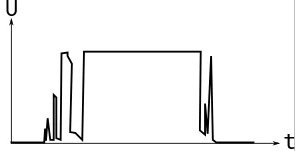
\includegraphics[scale=1.5]{chatter.png}
    \caption{Схематичное изображение дребезга на временной диаграмме}
    \label{fig:chatter}
\end{figure}

Как правило, считается, что контакт в переключателе является надежным и срабатывает мгновенно~\cite{sym}.

Однако на практике все несколько иначе. В каждом положении переключателя контакт между токопроводящими участками устанавливается или прерывается с помощью подвижных механических элементов.

Дребезг контактов возникает при нажатии на кнопку и переключатель из-за реальных вибраций контактной пластины при её перемещении. Как правило, пружинные компоненты применяются в качестве средства для перевода контакта из одного состояния в другое в виде либо металлической пластины, либо винтовой пружины. В тот момент, когда эти небольшие компоненты приводятся в движение, они перемещаются в требуемое положение. После срабатывания некоторое время происходят многократные неконтролируемые замыкания и размыкания контактов за счет упругости пружины и деталей контактной системы; при этом электрическая цепь размыкается и замыкается, пока движение полностью не прекратится~\cite{samel}.

В механических переключателях применяются механические же способы уменьшения дребезга контактов. Но полностью решить проблему они не могут. Наиболее часто применяют так называемый <<механизм мгновенного действия>>. Пример того, как такой механизм может выглядеть представлен на Рис.~1.2~\cite{dzen}.

\begin{figure}[H]
    \centering
    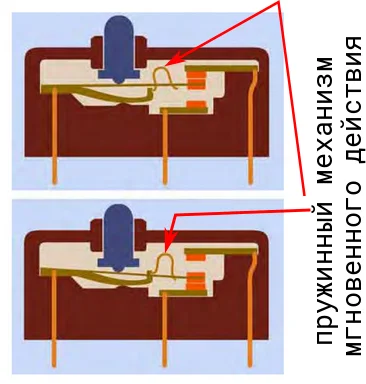
\includegraphics[scale=1.2]{instant_action.png}
    \caption{Механизм мгновенного действия}
    \label{fig:instant_action}
\end{figure}

При этом, в процессе эксплуатации кнопки <<стареют>>. Контакты изнашиваются и загрязняются, а дребезг и переходное сопротивление возрастают.

Время и характер дребезга контактов очень сильно зависят о конкретного механического переключателя (размеры, конструкция, назначение) и степени его износа (время эксплуатации). Обычно, время дребезга составляет единицы, реже, десятки миллисекунд. Но может достигать и сотен миллисекунд для больших переключателей.

\chapter{Устранение эффекта дребезга контактов}

Для подавления дребезга контактов в электронных схемах существует два пути:

\begin{enumerate}
    \item Решение программным путем

    \begin{enumerate}
        \item Использование задержек
    
        \item Использование счетчиков
    
        \item Использование прерываний по состоянию вывода порта
    \end{enumerate}

    \item Решение аппаратным путем

    \begin{enumerate}
        \item Сглаживающие фильтры
    
        \item Триггер Шмидта
    
        \item Использование одновибратора (ждущего мультивибратора)
    \end{enumerate}
\end{enumerate}

\section{Программные решения}

\subsection{Использование задержек}

Самым простым способом справиться с проблемой дребезга кнопки является выдерживание паузы. Микроконтроллер останавливается и ждет, пока переходный процесс не завершится. Для этого можно использовать любую встроенную функцию задержки, интегрированную в язык программирования. 10-50 миллисекунд обычно для большинства случаев.

Проблема с дребезгом настолько популярна, что есть специальные библиотеки, в которых не надо организовывать ожидание и паузы вручную --- это все делается внутри специального класса. Пример популярной библиотеки для борьбы с дребезгом кнопок --- библиотека Bounce.

В приложении приведен пример программы, которая реализует данный метод подавления дребезга.

\subsection{Использование циклического опроса и счетчиков}

Данный способ представляет собой циклическое считывание состояния кнопки с установленным интервалом считывания (обычно примерно 0,5-5 мс). Эта операция может выполняться как внутри основного цикла программы, так и в процедуре обработки прерываний таймера, которые будут происходить с той же частотой.

Основу этого метода составляет счетчик связанный с циклом опроса кнопки. В начальном состоянии он равен 0. Если в очередном цикле опроса кнопки на выводе порта высокий уровень, а значение счетчика еще не достигло порогового значения, счетчик инкрементируется. Если в очередном цикле опроса кнопки на выводе порта низкий уровень, а счетчик не равен 0, то он декрементируется.

Достижение счетчиком порогового значения свидетельствует о том, что за последние циклы опроса состояние кнопки не изменялось и она нажата. Достижение счетчиком нулевого значения свидетельствует о том, что за последние циклы опроса состояние кнопки не изменялось и она отпущена.

\subsection{Использование прерываний по состоянию вывода порта}

Это более сложный способ обработки кнопки. К тому же, не в каждом микроконтроллере есть прерывания вообще, и по изменению состояния порта, в частности. Зато этот метод позволяет сразу фиксировать моменты нажатия и отпускания. Кроме того, программе на нужно тратить время на сканирование кнопки.

Собственно говоря, это одна из реализаций способа с использованием задержек.

Микроконтроллер запоминает состояние, 0 или 1, для заданного вывода порта. Когда состояние меняется, не важно, из 0 в 1, или из 1 в 0, микроконтроллер генерирует прерывание. В некоторых случаях можно задавать какое изменение (0-1 или 1-0) генерирует прерывание. Дополнительно может потребоваться выполнять чтение порта, для обновления сохраненной информации о состоянии вывода.

В начальный момент времени считается, что кнопка не нажата. При этом прерывания по изменению состояния вывода порта разрешены.

Как только состояние вывода изменится, микроконтроллер сгенерирует прерывание. Если состояние вывода изменилось из 0 в 1, мы фиксируем нажатие кнопки. Если состояние изменилось из 1 в 0, мы фиксируем отпускание кнопки.

При этом прерывания по изменению состояния вывода порта нужно заблокировать на время гашения дребезга контактов. Это исключает влияние дребезга на состояние кнопки в программе.

По истечении заданного времени гашения дребезга снова разрешаются прерывания по изменению состояния вывода порта.

Далее, обработка кнопки будет проходить так же, как и в начальный момент времени. С той лишь разницей, что теперь у нас не предопределенное (отпущена), а фактическое состояние кнопки.

В приложении приведен алгоритм работы такого метода и программный код в качестве примера.

\section{Аппаратные решения}

\subsection{Сглаживающие фильтры}

Один из аппаратных способов устранения дребезга основан на использовании сглаживающих фильтров~\cite{prog}.

Это очень популярный метод гашения дребезга. Большинство используемых кнопок имеют лишь контакт на замыкание, что не позволяет использовать RS-триггер.

Сглаживающий фильтр занимается сглаживанием всплесков сигналов за счет добавления в схему элементов, имеющих своеобразную <<инерцию>> по отношению к таким электрическим параметрам как ток или напряжение. Самым распространенным примером таких <<инерционных>> электронных компонентов является конденсатор. Он может медленно накапливать и отдавать энергию, что позволяет добиться сглаживания~\cite{dzen}.

Пример простого фильтра на базе RC-цепочки представлен на Рис.~2.1.

\begin{figure}[H]
    \centering
    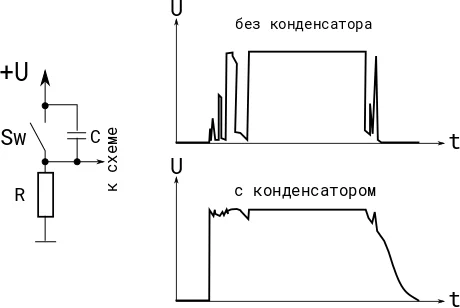
\includegraphics{capasitor.png}
    \caption{Сглаживающий фильтр}
    \label{fig:capasitor}
\end{figure}

Когда кнопка не нажата конденсатор заряжен, поэтому ток в цепи не протекает и не создает падения напряжения на резисторе. На входе схемы низкий уровень напряжения. Нажатие кнопки разряжает конденсатор. При этом на входе схемы появляется напряжение высокого уровня, через контакты кнопки. Короткие периоды разомкнутого состояния контактов во время дребезга позволяют конденсатору немного зарядиться через резистор, при этом протекающий через резистор тока заряда конденсатора создает на нем падение напряжения, а это поддерживает на входе схемы напряжение высокого уровня, но плавно спадающее.

Если постоянная времени RC цепи выбрана правильно, конденсатор не успевает заметно зарядиться за время дребезга, что позволяет избежать ошибочной работы схемы, к которой кнопка подключена~\cite{asutpp}.

Этот метод гашения дребезга позволяет точно отследить момент замыкания кнопки, но момент размыкания отслеживается с задержкой. А это может быть критично. Кроме того, быстрое отпускание и повторное нажатие кнопки может быть воспринято как единичное длительное нажатие, так как конденсатор не успеет зарядиться до уровня, когда будет зафиксирован логический 0.

Сделать квадратную форму сигнала с помощью простой RC цепочки невозможно. Для <<огранения>> сглаженных форм используется триггер Шмидта, который срабатывает при достижении определенного уровня сигнала. На выходе триггера Шмидта мы получим или высокий или низкий уровень сигнала. Ниже представлена схема и результат работы с триггером Шмидта~\cite{arduino}.

Устранение дребезга с помощью триггера Шмидта представлено на Рис.~2.2.

\begin{figure}[H]
    \begin{minipage}[h]{0.49\linewidth}
    \center{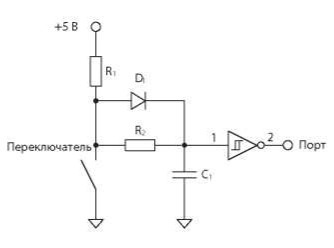
\includegraphics[width=1.15\linewidth]{trigger.jpg}}
    \end{minipage}
    \hfill
    \begin{minipage}[h]{0.49\linewidth}
    \center{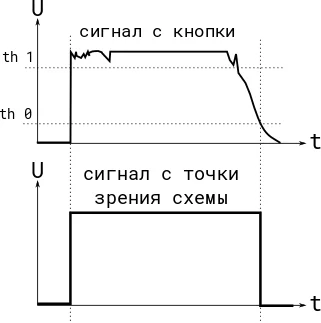
\includegraphics[width=0.75\linewidth]{shmidt.png}}
    \end{minipage}
    \caption{Устранение дребезга с помощью триггера Шмидта}
    \label{fig:image1}
\end{figure}

\subsection{RS-триггер}

Это классический и давно используемый метод. Схема для борьбы с дребезгом представлена на Рис.~2.3.

\begin{figure}[H]
    \centering
    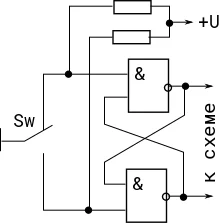
\includegraphics[scale=1.5]{RS.png}
    \caption{Схема для подавления дребезга с использованием RS-триггеров}
    \label{fig:rs}
\end{figure}

Эта схема гарантированно подавляет дребезг. Но она требует использования кнопки с переключающим контактом. Конструкция кнопки с переключающим контактом такова, что дребезг сразу двух половин контактной группы исключен. Именно это исключает многократное опрокидывание триггера при нажатии и отпускании кнопки~\cite{dzen}.

Эта схема не фиксирует момент размыкания верхнего контакта, она фиксирует момент первого замыкания нижнего контакта. Точно так же, она не фиксирует момент размыкания нижнего контакта, но фиксирует момент замыкания верхнего. Учет этой особенности иногда может быть важным, когда кнопка используется для отслеживания положения объекта, а не нажимается человеком.

\subsection{Использование одновибратора (ждущего мультивибратора)}

Этот метод тоже встречается, хотя и реже двух ранее описанных. Пример схемы и ее работы представлен на Рис.~2.4.

\begin{figure}[H]
    \centering
    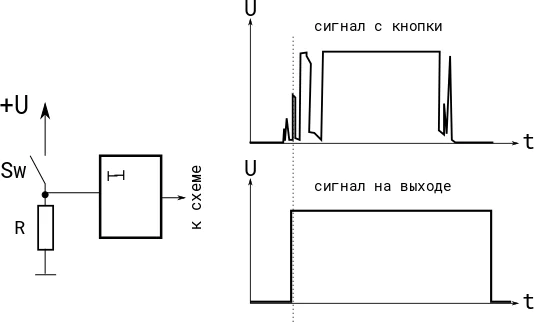
\includegraphics{vibrator.png}
    \caption{Использование одновибратора для подавления дребезга}
    \label{fig:vib}
\end{figure}

Одновибратор может быть перезаускаемым, или не перезапускаемым. В данном случае, он запускается по переднему фронту первого, распознанного как переход от низкого к высокому уровню, импульса. И выдает на выходе импульс фиксированной длительности, не зависящей от длительности нажатия кнопки~\cite{dzen}.

Одновибратор может быть и специализированной микросхемой, и реализован, например, на D-триггере.

Однако, данный метод гашения дребезга имеет один, но существенный, недостаток. Если длительность нажатия кнопки больше длительности формируемого импульса, то возможны ложные срабатывания дребезга при отпускании кнопки. Кроме того, можно отследить только момент нажатия кнопки, но не момент отпускания.

Схему можно усложнить, что позволит устранить некоторые недостатки. Можно использовать несколько одновибраторов, что позволит сформировать отдельный сигнал длинного нажатия, а это невозможно с приведенными выше методами. Однако, в настоящее время такие решения применяются довольно редко.

\chapter{Борьба с дребезгом в реальном проекте}

Среди рассмотренных ранее методов для конкретного проекта наиболее подходящим является аппаратный метод подавления дребезга с использованием прерываний по состоянию вывода порта.

Преимуществом данного метода по сравнению с любым аппаратным является тот факт, что для использования данного метода не нужно вносить никаких изменений в схему устройства, что в свою очередь не ведет к ее удорожанию и другим проблемам, к которым может привести добавление новых элементов.

Преимущество данного метода перед другими программными реализациями заключается в том, что, по сравнению с использованием обычной задержки, не требуется останавливать работу микроконтроллера, чтобы дождаться окончания дребезга, а также программа не будет тратить время на постоянный опрос состояния кнопки, как при использовании счетчика.

В Arduino для таких целей предусмотрен метод attachInterrupt, одним из параметров которого является функция, в которой прописываются действия, которые должны выполниться для обработки прерывания после его генерации.

В приложении приведен код программы с реализацией данного метода. Алгоритм подавления дребезга представлен на Рис.~3.1.

\begin{figure}[H]
    \centering
    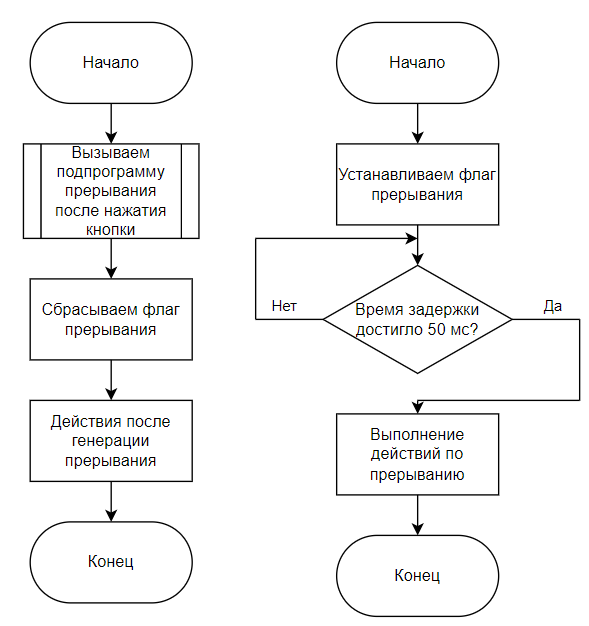
\includegraphics[scale=0.6]{algorithm.png}
    \caption{Алгоритм подавления дребезга с помощью прерываний}
    \label{fig:alg}
\end{figure}

\newpage
\addcontentsline{toc}{chapter}{Список использованной литературы}
\printbibliography[title={Список использованной литературы}]

\chapter*{Приложение}
\addcontentsline{toc}{chapter}{Приложение}

\begin{code}
\captionof{listing}{Исходный код для иллюстрации метода задержек}
\label{code:pi-example}
\begin{minted}[mathescape,linenos,frame=lines,breaklines]{C++}
int currentValue, prevValue;
void loop() {
  currentValue = digitalRead(PIN_BUTTON);
  if (currentValue != prevValue) {
    // Место, где возможна зона неопределенности
    // Делаем задержку 50 мс
    delay(50);
    // Считываем значение, считая, что нестабильность исчезла
    currentValue = digitalRead(PIN_BUTTON);
  }

  prevValue = currentValue;
  Serial.println(currentValue);
}
\end{minted}
\end{code}

\begin{code}
\captionof{listing}{Исходный код для иллюстрации метода циклического опроса и счетчиков}
\label{code:pi-example}
\begin{minted}[mathescape,linenos,frame=lines,breaklines]{C++}
// Состояния кнопки

bool KeyPressed; // Кнопка нажата
int KeyCounter; // Счетчик кнопки
int LongCounter; // Счетчик длительного нажатия

// События кнопки

bool ShortPress; // короткое нажатие
bool LongPress; // Длинное нажатие

// Пороги состояний кнопки

int Press_th; // Порог гашения дребезга
int Long_th; // Порог длинного нажатия

// Вывод порта к которому подключена кнопка

bool key;

// Начальные значения переменных

KeyPressed = false;
KeyCounter = 0:
LongCounter = 0;
ShortPress = false;
LongPress = false;
ShortPress = false;

if(Key) {
    if (KeyConter < Press_th) {
        KeyCounter++;
    } else { 
        KeyPresed=true; 
        if (LongCounter < Long_th) {
            LongCounter++; 
        } else{ 
            Longpress=true;
        }
} else {
    if (KeyCounter) {
        KeyCounter--;
    } else { 
        KeyPressed=false; 
        LongCounter=0; 
        if(!LongPress) {
            ShortPress=true; 
        } else { 
            LongPress=false;
        }
    }
}
\end{minted}
\end{code}

\begin{code}
\captionof{listing}{Исходный код для иллюстрации метода прерываний по состоянию вывода порта}
\label{code:pi-example}
\begin{minted}[mathescape,linenos,frame=lines,breaklines]{C++}
volatile boolean chatterFlag = false; 
 
void setup() {
  Serial.begin(9600);
  pinMode(2, INPUT_PULLUP); 
  attachInterrupt(0, chatter, FALLING);
}
 
volatile uint32_t chatter_time;
void chatter() {
  chatterFlag = true;
  // 50 подавляем дребезг кнопки, читаем состояние порта
  if (millis() - chatter_time >= 50 && digitalRead(2))
  {
    chatter_time = millis();
    // Дальнейший код прерывания
  }
}
 
void loop() {
  if (chatterFlag) {
    chatterFlag = false;    
    // Действия после генерации прерывания
  } 
    delay(1000);              
}
\end{minted}
\end{code}

\begin{figure}[H]
    \centering
    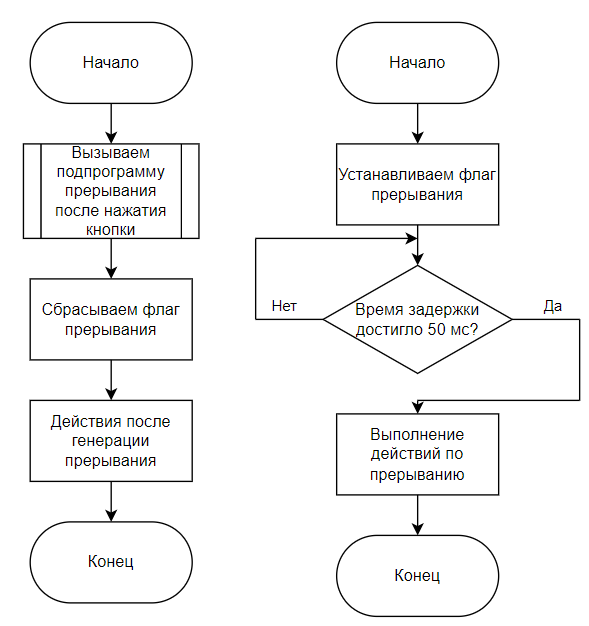
\includegraphics[scale=0.6]{algorithm.png}
    \caption{Алгоритм подавления дребезга с помощью прерываний}
    \label{fig:alg}
\end{figure}

\end{document}